\documentclass[a4paper,10pt]{article}
\linespread{1.25}
\usepackage{cmap}
\usepackage[T2A]{fontenc}
\usepackage[utf8x]{inputenc}
\usepackage[english,russian]{babel}
\usepackage{mathtools}
\usepackage{amsmath,array}
\newcommand{\diff}{\mathop{}\!d} % thanks egreg
\usepackage[left=2cm,right=2cm,
top=2cm,bottom=2cm,bindingoffset=0cm]{geometry}
\usepackage{amsfonts} 
\usepackage{longtable}
\usepackage{blindtext}
\usepackage{listings}
\usepackage{xcolor}
\lstdefinestyle{sharpc}{language=[Sharp]C, frame=lr, rulecolor=\color{blue!80!black}}
\usepackage{xltabular}
\usepackage{lstfiracode}
\usepackage{graphicx}
\usepackage{float}%"Плавающие" картинки
\usepackage{wrapfig}%Обтекание фигур (таблиц, картинок и прочего)
\graphicspath{{pictures/}}
\DeclareGraphicsExtensions{.pdf,.png,.jpg}
\usepackage{tikz}
\usetikzlibrary{automata, positioning}

\lstset{ %
	language=[Sharp]C,                 % выбор языка для подсветки (здесь это С)
	basicstyle=\small\sffamily, % размер и начертание шрифта для подсветки кода
	numbers=left,               % где поставить нумерацию строк (слева\справа)
	numberstyle=\tiny,           % размер шрифта для номеров строк
	stepnumber=1,                   % размер шага между двумя номерами строк
	numbersep=5pt,                % как далеко отстоят номера строк от подсвечиваемого кода
	backgroundcolor=\color{white}, % цвет фона подсветки - используем \usepackage{color}
	showspaces=false,            % показывать или нет пробелы специальными отступами
	showstringspaces=false,      % показывать или нет пробелы в строках
	showtabs=false,             % показывать или нет табуляцию в строках
	frame=single,              % рисовать рамку вокруг кода
	tabsize=2,                 % размер табуляции по умолчанию равен 2 пробелам
	captionpos=t,              % позиция заголовка вверху [t] или внизу [b] 
	breaklines=true,           % автоматически переносить строки (да\нет)
	breakatwhitespace=false, % переносить строки только если есть пробел
	escapeinside={\%*}{*)}   % если нужно добавить комментарии в коде
}

\begin{document}
	\begin{titlepage}
		\begin{center}
			\textsc{Московский авиационный институт \\[2mm]
				(национальный исследовательский университет) 
				\textcolor{blue}{\noindent\makebox[\linewidth]{\rule{\textwidth}{0.4pt}}}\\[5mm]
				Институт «Компьютерные науки и прикладная математика»}
			\vfill
			\textbf{Лабораторные работы\\[2mm]
				по курсу \\[3mm]
				«Системы программирования»\\[2mm]
				IV семестр
				\\[5mm]
			}
		\end{center}
		\begin{enumerate}
			\item Спроектировать грамматику по паттерн-модели регулярного языка.
			\item Преобразовать спроектированную грамматику в конечный автомат, составить диаграмму переходов КА и  реализовать.
			\item Определить свойства КА. Изучить  алгоритм преобразования НДКА в ДКА. \\[1mm]
			\item Устранить из КС-грамматики  бесполезные символы и $ \varepsilon $–правила.
			\item Устранить из KС-грамматики цепные правила и устранить левую рекурсию.
			\item Определить форму КС-грамматики и сделать ее приведение.
			\item Спроектировать МП-автомат для приведенной КС-грамматики.
			\item Реализовать МП-автомат для приведенной КС-грамматики. \\[1mm]
			\item Для LL(k) анализатора построить управляющую таблицу M.
			\item Аналитически написать правила вывода для цепочки LL(k) анализатора.
			\item Реализовать управляющую таблицу M Для LL(k) анализатора. \\[1mm]
			\item Построить множество LR(0)-таблиц не содержащих $ \varepsilon $–правила.
			\item Для LR(k)-грамматики cпроектировать матрицу oblow.
			\item Определить функции перехода g(X).
			\item Определить функцию переноса-свертки f(u).
			\item Для функции перехода g(X) и функции переноса-свертки f(u) спроектировать управляющую таблицу.
		\end{enumerate}
		\vfill
		\hfill
		\begin{minipage}{.3\textwidth}
			\textit{Студент}: Павлов И.Д.\\
			\textit{Группа}: М8О-207Б-21\\
			\textit{Руководитель}: Семенов А.С.
		\end{minipage}%
		\vfill
		\begin{center}
			\textbf{Москва, 2023}
		\end{center}
	\end{titlepage}
	
	\newpage
	
	\begin{center}
		\textbf{Практическая работа №1 (1-3 лаб.)}
	\end{center}
	\underline{\textit{Лабораторные работы №1-2}} \\[5mm]
	\textbf{Формулировка задания:} \\[3mm]
	\hspace*{5mm} Спроектировать грамматику для двух заданных паттернов. Составить на основе разработанных регулярных грамматик конечные автоматы, распознающие эквивалентные им языки. \\
	\begin{center}
		\textbf{1}. \textbf{pattern = "192$\backslash$.168$\backslash$.1$\backslash$.$\backslash$d\{1, 3\}" }
	\end{center}
	\textbf{Автоматная грамматика:} \\[3mm]
	\hspace*{5mm} $L($pattern$)$ = $L($"192$\backslash$.168$\backslash$.1$\backslash$.$\backslash$d\{1, 3\}"$)$ = $\{$"192.168.1.0"\ ,\dots, "192.168.1.999"$\}$ \\
	\hspace*{5mm} $G(T, V, P, S_0) = G(\{0, \dots, 9, .\}, \{S_0, A, \dots, M\}, \{p_1, p_2, \dots, p_{16}\}, S_0)$ \\[5mm]
	\textit{Правила регулярной грамматики:}
	\begin{itemize}
		\item[\textbf{p1:}] $S_0 \to 1A$
		\item[\textbf{p2:}] $A \to 9B$
		\item[\textbf{p3:}] $B \to 2C$
		\item[\textbf{p4:}] $C \to . D$
		\item[\textbf{p5:}] $D \to 1E$
		\item[\textbf{p6:}] $E \to 6F$
		\item[\textbf{p7:}] $F \to 8G$
		\item[\textbf{p8:}] $G \to .H$
		\item[\textbf{p9:}] $H \to 1I$
		\item[\textbf{p10:}] $I \to .J$
		\item[\textbf{p11:}] $J \to 0K \hspace{2mm} | \hspace{2mm} 1K \hspace{2mm} |\hspace{2mm} \dots \hspace{2mm}|\hspace{2mm} 9K$
		\item[\textbf{p12:}] $K \to \varepsilon$
		\item[\textbf{p13:}] $K \to 0L \hspace{2mm} | \hspace{2mm} 1L \hspace{2mm} |\hspace{2mm} \dots \hspace{2mm}|\hspace{2mm} 9L$
		\item[\textbf{p14:}] $L \to \varepsilon$
		\item[\textbf{p15:}] $L \to 0M \hspace{2mm} | \hspace{2mm} 1M \hspace{2mm} |\hspace{2mm} \dots \hspace{2mm}|\hspace{2mm} 9M$
		\item[\textbf{p16:}] $M \to \varepsilon$
	\end{itemize}
	\vspace*{5mm}
	\textit{Пример цепочек:}
	\begin{itemize}
		\item[] $S_0 \rightarrow^{1} 1A \rightarrow^{2} 19B \rightarrow^{3} 192C \rightarrow^{4} 192.D \rightarrow^{5} 192.1E \rightarrow^{6} 192.16F \rightarrow^{7} 192.168G \rightarrow^{8} 192.168.H \rightarrow^{9} 192.168.1I \rightarrow^{10} 192.168.1.J \rightarrow^{11} 192.168.1.1K \rightarrow^{12} 192.168.1.1$
		\item[] $S_0 \rightarrow^{1} 1A \rightarrow^{2} 19B \rightarrow^{3} 192C \rightarrow^{4} 192.D \rightarrow^{5} 192.1E \rightarrow^{6} 192.16F \rightarrow^{7} 192.168G \rightarrow^{8} 192.168.H \rightarrow^{9} 192.168.1I \rightarrow^{10} 192.168.1.J \rightarrow^{11} 192.168.1.2K \rightarrow^{13} 192.168.1.25L \rightarrow^{15} 192.168.1.255M \rightarrow^{16} 192.168.1.255$  
	\end{itemize}
	
	\newpage
	
	\text{} \\
	\textbf{Конечный автомат:} \\[3mm]
	\hspace*{5mm} $L(KA) = L(G)$ \\[2mm]
	\hspace*{5mm} $KA = (Q, \varSigma, \delta, S_0, F)$, где \\[2mm]
	\hspace*{5mm} $Q = \{ S_0, A, \dots, M, q_f \}$, $\varSigma = \{ 0, 1, \dots, 9, . \}$, $S_0=S_0$, $F=\{ K, L, M \}$, \\[2mm]
	\hspace*{5mm} $\delta = \{ $
	\begin{align*}
		1. \hspace{2mm} \delta(S_0, 1) &= \{A\} & 2. \hspace{2mm} \delta(A, 9) &= \{B\}  \\ 
		3. \hspace{2mm} \delta(B, 2) &= \{C\} & 4. \hspace{2mm} \delta(C, .) &= \{D\}  \\
		5. \hspace{2mm} \delta(D, 1) &= \{E\} & 6. \hspace{2mm} \delta(E, 6) &= \{F\}  \\
		7. \hspace{2mm} \delta(F, 8) &= \{G\} & 8. \hspace{2mm} \delta(G, .) &= \{H\}  \\
		9. \hspace{2mm} \delta(H, 1) &= \{I\} & 10. \hspace{2mm} \delta(I, .) &= \{J\}  \\
		11. \hspace{2mm} \delta(J, 0) &= \{K\} & \dots  \\
		19. \hspace{2mm} \delta(J, 9) &= \{K\} & 20. \hspace{2mm} \delta(K, \varepsilon) &= \{K\} \\
		21. \hspace{2mm} \delta(K, 0) &= \{L\} & \dots \\
		30. \hspace{2mm} \delta(K, 9) &= \{L\} & 31. \hspace{2mm} \delta(L, \varepsilon) &= \{L\} \\
		32. \hspace{2mm} \delta(L, 0) &= \{M\} & \dots \\
		41. \hspace{2mm} \delta(L, 9) &= \{M\} & 42. \hspace{2mm} \delta(M, \varepsilon) &= \{M\}
	\end{align*}
	\hspace*{5mm} $\}$ \\[5mm]
	\textit{Примеры конфигурации КА:}
	\begin{enumerate}
		\item $(S_0, 192.168.1.1) \vdash^{1} (A, 92.168.1.1) \vdash^{2} (B, 2.168.1.1) \vdash^{3} (C, .168.1.1) \vdash^{4} (D, 168.1.1) \vdash^{5} (E, 68.1.1) \vdash^{6} (F, 8.1.1) \vdash^{7} (G, .1.1) \vdash^{8} (H, 1.1) \vdash^{9} (I, .1) \vdash^{10} (J, 1) \vdash^{12} (K, \varepsilon) \vdash^{20} (q_f, \varepsilon)$
		\item $(S_0, 192.168.1.255) \vdash^{1} (A, 92.168.1.255) \vdash^{2} (B, 2.168.1.255) \vdash^{3} (C, .168.1.255) \vdash^{4} (D, 168.1.255) \vdash^{5} (E, 68.1.255) \vdash^{6} (F, 8.1.255) \vdash^{7} (G, .1.255) \vdash^{8} (H, 1.255) \vdash^{9} (I, .255) \vdash^{10} (J, 255) \vdash^{13} (K, 55) \vdash^{26} (L, 5) \vdash^{37} (M, \varepsilon) \vdash^{42} (q_f, \varepsilon)$
	\end{enumerate}
	\vspace*{5mm}
		\begin{center}
		\begin{tikzpicture}[->,shorten >=1pt,auto,node distance=1.9cm,]
			\tikzstyle{state}=[draw,circle]
			
			\node[state] (S0) {$S_0$};
			\node[state] (A) [above right of=S0] {$A$};
			\node[state] (B) [below right of=A] {$B$};
			\node[state] (C) [below right of=S0] {$C$};
			\node[state] (D) [right of=C] {$D$};
			\node[state] (E) [right of=D] {$E$};
			\node[state] (F) [right of=E] {$F$};
			\node[state] (G) [below right of=F] {$G$};
			\node[state] (H) [above right of=F] {$H$};
			\node[state] (I) [right of=H] {$I$};
			\node[state] (J) [above right of=I] {$J$};
			\node[state, accepting] (K) [above right of=J] {$K$};
			\node[state, accepting] (L) [above left of=K] {$L$};
			\node[state, accepting] (M) [above right of=L] {$M$};
			
			\path (S0) edge node {1} (A)
			(A) edge node {9} (B)
			(B) edge node {2} (C)
			(C) edge node {$\dot{}$} (D)
			(D) edge node {1} (E)
			(E) edge node {6} (F)
			(F) edge node {8} (G)
			(G) edge node {$\dot{}$} (H)
			(H) edge node {1} (I)
			(I) edge node {$\dot{}$} (J)
			(J) edge node {[0-9]} (K)
			(K) edge node {[0-9]} (L)
			(L) edge node {[0-9]} (M);
		\end{tikzpicture}
	\end{center}
	\vspace*{5mm}
	\textit{Лемма о накачке:}
	\vspace*{5mm}
	\begin{center}
		$\forall L \subseteq \sum^{*} (regular(L)) \Rightarrow$ \\
		$( \exists p \ge 1 $ \\
		$(\forall w \in L ((\|w\| \ge p) \Rightarrow $ \\
		$( \exists x, y, z \in \sum^{*} (w = xyz \Rightarrow$ \\
		$(\|y\| \ge 1 \wedge \|xy\| \le p \wedge i \ge 0 \wedge (xy^{i}z \in L )) $ \\
		$)))))) $\\
	\end{center}
	\vspace*{5mm}
	\begin{figure}[h]
		\centering
		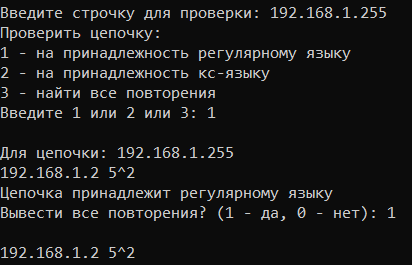
\includegraphics[]{1.png}
		\label{fig:mpr}
	\end{figure}
	\vspace*{5mm}
	\begin{center}
		\textbf{2}. \textbf{pattern = "(?i)($\backslash$W|$\wedge$)(baloney|darn|drat|fooey|gosh$\backslash$sdarnit|heck)($\backslash$W|\$)" }
	\end{center}
	\textbf{Автоматная грамматика:} \\[3mm]
	\hspace*{5mm} $L($pattern$)$ = $L("(?i)(\backslash W|\wedge)(baloney|darn|drat|fooey|gosh \backslash sdarnit|heck)( \backslash W|\$)"$)$ = $ \\
	\hspace*{5mm}$=$ $\{$"baloney"{}, "Baloney"{} , \dots $\}$ \\
	\hspace*{5mm} $G(T, V, P, S_0) = G(\{B, b, A, a, L, l, O, o, N, n, E, e, Y, y, D, d, R, r, N, n, T, t, F, f, G, g, S, s, H, h, \backslash s, I, i, C, c, \backslash W\}$,
	\hspace*{5mm}$ \{S_0, A, \dots, Z, AA, q_f\}, \{p_1, p_2, \dots, p_{34}\}, S_0)$, \\\hspace*{5mm}где $\backslash W$ это все символы, не являющиеся буквой и цифрой; $\backslash s$ это пробел \\[5mm]
	
		\textit{Правила регулярной грамматики:}
	\begin{itemize}
		\item[\textbf{p1:}] $S_0 \to \backslash WS_0$
		\item[\textbf{p2:}] $S_0 \to bA \hspace{2mm} | \hspace{2mm} BA$
		\item[\textbf{p3:}] $S_0 \to dG \hspace{2mm} | \hspace{2mm} DG$
		\item[\textbf{p4:}] $S_0 \to gO \hspace{2mm} | \hspace{2mm} GO$
		\item[\textbf{p5:}] $S_0 \to fL \hspace{2mm} | \hspace{2mm} FL$
		\item[\textbf{p6:}] $S_0 \to hY \hspace{2mm} | \hspace{2mm} HY$
		\item[\textbf{p7:}] $A \to aB \hspace{2mm} | \hspace{2mm} AB$
		\item[\textbf{p8:}] $B \to lC \hspace{2mm} | \hspace{2mm} LC$
		\item[\textbf{p9:}] $C \to oD \hspace{2mm} | \hspace{2mm} OD$
		\item[\textbf{p10:}] $D \to nE \hspace{2mm} | \hspace{2mm} NE$
		\item[\textbf{p11:}] $E \to eF \hspace{2mm} | \hspace{2mm} EF$
		\item[\textbf{p12:}] $F \to yq_{f} \hspace{2mm} | \hspace{2mm} Yq_{f}$
		\item[\textbf{p13:}] $G \to aH \hspace{2mm} | \hspace{2mm} AH$
		\item[\textbf{p14:}] $G \to rJ \hspace{2mm} | \hspace{2mm} RJ$
		\item[\textbf{p15:}] $H \to rI \hspace{2mm} | \hspace{2mm} RI$
		\item[\textbf{p16:}] $I \to nq_{f} \hspace{2mm} | \hspace{2mm} Nq_{f}$
		\item[\textbf{p17:}] $J \to aK \hspace{2mm} | \hspace{2mm} AK$
		\item[\textbf{p18:}] $K \to tq_{f} \hspace{2mm} | \hspace{2mm} Tq_{f}$
		\item[\textbf{p19:}] $L \to oM \hspace{2mm} | \hspace{2mm} OM$
		\item[\textbf{p20:}] $M \to oE \hspace{2mm} | \hspace{2mm} OE$
		\item[\textbf{p21:}] $O \to oP \hspace{2mm} | \hspace{2mm} OP$
		\item[\textbf{p22:}] $P \to sQ \hspace{2mm} | \hspace{2mm} SQ$
		\item[\textbf{p23:}] $Q \to hR \hspace{2mm} | \hspace{2mm} HR$
		\item[\textbf{p24:}] $R \to \backslash sS $
		\item[\textbf{p25:}] $S \to dT \hspace{2mm} | \hspace{2mm} DT$
		\item[\textbf{p26:}] $T \to aU \hspace{2mm} | \hspace{2mm} AU$
		\item[\textbf{p27:}] $U \to rV \hspace{2mm} | \hspace{2mm} RV$
		\item[\textbf{p28:}] $V \to nW \hspace{2mm} | \hspace{2mm} NW$
		\item[\textbf{p29:}] $W \to iX \hspace{2mm} | \hspace{2mm} IX$
		\item[\textbf{p30:}] $X \to tQ_{f} \hspace{2mm} | \hspace{2mm} Tq_{f}$
		\item[\textbf{p31:}] $Y \to eZ \hspace{2mm} | \hspace{2mm} EZ$
		\item[\textbf{p32:}] $Z \to cAA \hspace{2mm} | \hspace{2mm} CAA$
		\item[\textbf{p33:}] $AA \to kq_{f} \hspace{2mm} | \hspace{2mm} KAG$
		\item[\textbf{p34:}] $q_f \to \backslash Wq_{f} \hspace{2mm} | \hspace{2mm} \varepsilon$
		
	\end{itemize}
	\vspace*{5mm}
	\textit{Пример цепочек:}
	\begin{itemize}
		\item[] $S_0 \rightarrow^{1} !S_0 \rightarrow^{2} !BA \rightarrow^{7} !BaB \rightarrow^{8} !BaLC
		\rightarrow^{9} !BaLOD \rightarrow^{10} !BaLOnE \rightarrow^{11} !BaLOnEF \rightarrow^{12} !BaLOnEy$
		\item[] $S_0 \rightarrow^{5} fL \rightarrow^{19} fOM \rightarrow^{20} fOoE \rightarrow^{11} fOoEF \rightarrow^{12} fOoEy $
	\end{itemize}
	
	
	\text{} \\
	\textbf{Конечный автомат:} \\[3mm]
	\hspace*{5mm} $L(KA) = L(G)$ \\[2mm]
	\hspace*{5mm} $KA = (Q, \varSigma, \delta, S_0, F)$, где \\[2mm]
	\hspace*{5mm} $Q = \{ S_0, A, \dots, Z, AA, q_f \}$, $\varSigma = \{ B, b, A, a, L, l, O, o, N, n, E, e, Y, y, D, d, R, r, N, n, T, t, F, f, G, g, S, s, H, h, \backslash s$,
	\\ \hspace*{5mm }$ I, i, C, c, \backslash W \}$, $S_0=S_0$, $F=q_f$, \\[2mm]
	\hspace*{5mm} $\delta = \{ $
	\begin{align*}
		1. \hspace{2mm} \delta(S_0, \backslash W) &= \{S_0\} & 2. \hspace{2mm} \delta(S_0, b) &= \{A\}  \\ 
		3. \hspace{2mm} \delta(S_0, B) &= \{A\} & 4. \hspace{2mm} \delta(S_0, d) &= \{G\}  \\
		5. \hspace{2mm} \delta(S_0, D) &= \{G\} & 6. \hspace{2mm} \delta(S_0, g) &= \{O\}  \\
		7. \hspace{2mm} \delta(S_0, G) &= \{O\} & 8. \hspace{2mm} \delta(S_0, f) &= \{L\}  \\
		9. \hspace{2mm} \delta(S_0, F) &= \{L\} & 10. \hspace{2mm} \delta(S_0, h) &= \{Y\}  \\
		11. \hspace{2mm} \delta(S_0, H) &= \{Y\} & 12. \hspace{2mm} \delta(S_0, H) &= \{Y\}  \\
		13. \hspace{2mm} \delta(A, a) &= \{B\} & 14. \hspace{2mm} \delta(A, A) &= \{B\} \\
		15. \hspace{2mm} \delta(B, l) &= \{C\} & 16. \hspace{2mm} \delta(B, L) &= \{C\} \\
		17. \hspace{2mm} \delta(C, o) &= \{D\} & 18. \hspace{2mm} \delta(C, O) &= \{D\} \\
		19. \hspace{2mm} \delta(D, n) &= \{E\} & 20. \hspace{2mm} \delta(D, N) &= \{E\} \\
		21. \hspace{2mm} \delta(E, e) &= \{F\} & 22. \hspace{2mm} \delta(E, E) &= \{F\} \\
		23. \hspace{2mm} \delta(F, y) &= \{q_f\} & 24. \hspace{2mm} \delta(E, Y) &= \{q_f\} \\
		25. \hspace{2mm} \delta(G, a) &= \{H\} & 26. \hspace{2mm} \delta(G, A) &= \{H\} \\
		27. \hspace{2mm} \delta(H, r) &= \{I\} & 28. \hspace{2mm} \delta(H, R) &= \{I\} \\
		29. \hspace{2mm} \delta(I, n) &= \{q_f\} & 30. \hspace{2mm} \delta(I, n) &= \{q_f\} \\
		31. \hspace{2mm} \delta(G, r) &= \{J\} & 32. \hspace{2mm} \delta(G, R) &= \{J\} \\
		33. \hspace{2mm} \delta(J, a) &= \{K\} & 34. \hspace{2mm} \delta(J, A) &= \{K\} \\
		35. \hspace{2mm} \delta(K, t) &= \{q_f\} & 36. \hspace{2mm} \delta(K, T) &= \{q_f\} \\
		37. \hspace{2mm} \delta(L, o) &= \{M\} & 38. \hspace{2mm} \delta(L, O) &= \{M\} \\
		39. \hspace{2mm} \delta(M, o) &= \{E\} & 40. \hspace{2mm} \delta(M, O) &= \{E\} \\
		41. \hspace{2mm} \delta(O, o) &= \{P\} & 42. \hspace{2mm} \delta(O, o) &= \{P\} \\
		43. \hspace{2mm} \delta(P, s) &= \{Q\} & 44. \hspace{2mm} \delta(P, S) &= \{Q\} \\
		45. \hspace{2mm} \delta(Q, h) &= \{R\} & 46. \hspace{2mm} \delta(Q, H) &= \{R\} \\
		47. \hspace{2mm} \delta(R, \backslash s) &= \{S\} & 48. \hspace{2mm} \delta(S, d) &= \{T\} \\
		49. \hspace{2mm} \delta(S, D) &= \{T\} & 50. \hspace{2mm} \delta(T, a) &= \{U\} \\
		51. \hspace{2mm} \delta(T, A) &= \{U\} & 52. \hspace{2mm} \delta(U, r) &= \{V\} \\
		53. \hspace{2mm} \delta(U, R) &= \{V\} & 54. \hspace{2mm} \delta(V, n) &= \{W\} \\
		55. \hspace{2mm} \delta(V, N) &= \{W\} & 56. \hspace{2mm} \delta(W, i) &= \{X\} \\
		57. \hspace{2mm} \delta(W, I) &= \{X\} & 58. \hspace{2mm} \delta(X, t) &= \{q_f\} \\
		59. \hspace{2mm} \delta(X, t) &= \{q_f\} & 60. \hspace{2mm} \delta(Y, e) &= \{Z\} \\
		61. \hspace{2mm} \delta(Y, E) &= \{Z\} & 62. \hspace{2mm} \delta(Z, c) &= \{AA\} \\
		63. \hspace{2mm} \delta(Z, C) &= \{AA\} & 64. \hspace{2mm} \delta(AA, k) &= \{q_f\} \\
		65. \hspace{2mm} \delta(AA, K) &= \{q_f\} & 66. \hspace{2mm} \delta(q_f, \backslash W) &= \{q_f\}
	\end{align*}
	\hspace*{5mm} $\}$ \\[5mm]
	
	\textit{Примеры конфигурации КА:}
	\begin{enumerate}
		\item $(S_0, !BaLOnEy) \vdash^{1} (S_0, BaLOnEy) \vdash^{3} (A, aLOnEy) \vdash^{13} (B, LOnEy) \vdash^{16} (C, OnEy) \vdash^{18} (D, nEy) \vdash^{19} (E, Ey) \vdash^{22} (F, y) \vdash^{23} (q_f, \varepsilon)$
	\end{enumerate}
	\vspace*{5mm}
	\begin{center}
		\begin{tikzpicture}[->,shorten >=1pt,auto,node distance=2cm,semithick]
			\node[initial,state] (start) {$S0$};
			\node[state] (q1) [above right of=start] {$A$};
			\node[state] (q2) [right of=q1] {$B$};
			\node[state] (q3) [right of=q2] {$C$};
			\node[state] (q4) [right of=q3] {$D$};
			\node[state] (q5) [right of=q4] {$E$};
			\node[state] (q6) [right of=q5] {$F$};
			\node[state] (q7) [right of=start] {$G$};
			\node[state] (q8) [right of=q7] {$H$};
			\node[state] (q9) [right of=q8] {$I$};
			\node[state] (q10) [below right of=q7] {$J$};
			\node[state] (q11) [right of=q10] {$K$};
			\node[state] (q12) [above right of=q1] {$L$};
			\node[state] (q13) [right of=q12] {$M$};
			\node[state] (q14) [below right of=start] {$O$};
			\node[state] (q15) [below right of=q14] {$P$};
			\node[state] (q16) [below right of=q15] {$Q$};
			\node[state] (q17) [below of=q16] {$R$};
			\node[state] (q18) [below of=q17] {$S$};
			\node[state] (q19) [right of=q18] {$T$};
			\node[state] (q20) [above of=q19] {$U$};
			\node[state] (q21) [above of=q20] {$V$};
			\node[state] (q22) [right of=q21] {$W$};
			\node[state] (q23) [right of=q22] {$X$};
			\node[state] (q24) [above of=q12] {$Y$};
			\node[state] (q25) [above right of=q13] {$Z$};
			\node[state] (q26) [above of=q6] {$AA$};
			\node[state, accepting] (final) [below right of=q6] {$q_f$};
			
			\path[->]
			(start) edge [bend right=20] node {bB} (q1)
			(start) edge [loop below] node {$\backslash W$} ()
			(q1) edge node {aA} (q2)
			(q2) edge node {lL} (q3)
			(q3) edge node {oO} (q4)
			(q4) edge node {nN} (q5)
			(q5) edge node {eE} (q6)
			(q6) edge [bend right=20] node {yY} (final)
			(start) edge node {dD} (q7)
			(q7) edge node {aA} (q8)
			(q8) edge node {rR} (q9)
			(q9) edge node {nN} (final)
			(q7) edge node {rR} (q10)
			(q10) edge node {aA} (q11)
			(q11) edge node {tT} (final)
			(start) edge [bend left=35] node {fF} (q12)
			(q12) edge node {oO} (q13)
			(q13) edge [bend left=20] node {oO} (q4)
			(start) edge node {gG} (q14)
			(q14) edge node {oO} (q15)
			(q15) edge node {sS} (q16)
			(q16) edge node {hH} (q17)
			(q17) edge node {$\backslash s$} (q18)
			(q18) edge node {dD} (q19)
			(q19) edge node {aA} (q20)
			(q20) edge node {rR} (q21)
			(q21) edge node {nN} (q22)
			(q22) edge node {iI} (q23)
			(q23) edge node {tT} (final)
			(start) edge [bend left=50] node {hH} (q24)
			(q24) edge node {eE} (q25)
			(q25) edge node {cC} (q26)
			(q26) edge [bend left=50] node {kK} (final)
			(final) edge [loop below] node {$\backslash W$} ();
		\end{tikzpicture}
	\end{center}
	\vspace*{5mm}
	\textit{Лемма о накачке:}
	\vspace*{5mm}
	\begin{center}
		$\forall L \subseteq \sum^{*} (regular(L)) \Rightarrow$ \\
		$( \exists p \ge 1 $ \\
		$(\forall w \in L ((\|w\| \ge p) \Rightarrow $ \\
		$( \exists x, y, z \in \sum^{*} (w = xyz \Rightarrow$ \\
		$(\|y\| \ge 1 \wedge \|xy\| \le p \wedge i \ge 0 \wedge (xy^{i}z \in L )) $ \\
		$)))))) $\\
	\end{center}
	\begin{figure}[h]
		\centering
		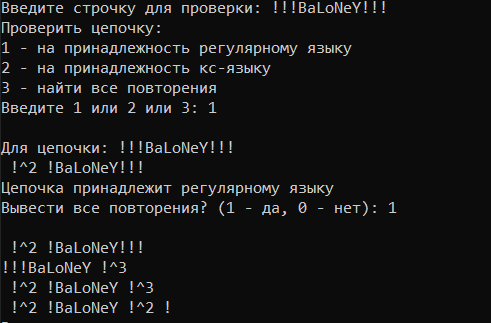
\includegraphics[]{2.png}
		\label{fig:mpr}
	\end{figure}
	\vspace*{5mm}
	
	\underline{\textit{Лабораторная работа №3}} \\[5mm]
	\textbf{Формулировка задания:} \\[3mm]
	\hspace*{5mm} Реализовать конечные автоматы, составленные в ЛР №2 \\
	
	\begin{lstlisting}
		FSAutomate[] automats = new FSAutomate[] {
			new FSAutomate(
			new List<Symbol>() { "S01", "A1", "B1", "C1", "D1", "E1", "F1", "G1",
				"H1", "I1", "J1", "K1", "L1", "M1" },
			new List<Symbol>() { "0", "1", "2", "3", "4", "5", "6", "7", "8", "9", "."  },
			new List<Symbol>() { "K1", "L1", "M1" },
			"S01"
			),
			new FSAutomate(
			new List<Symbol>() { "S02", "A2", "B2", "C2", "D2", "E2", "F2", "G2", "H2", "I2", "J2",
				"K2", "L2", "M2", "N2", "O2", "P2", "Q2", "R2", "S2", "T2", "U2",
				"V2", "W2", "X2", "Y2", "Z2", "AA2", "qf2"},
			new List<Symbol>() { "B", "b", "A", "a", "L", "l", "O", "o", "N", "n", "E", "e",
				"Y", "y", "D", "d", "R", "r", "N", "n", "T", "t", "F", "f",
				"G", "g", "S", "s", "H", "h", " ", "I", "i", "C", "c", @"\W" },
			new List<Symbol>() { "qf2" },
			"S02"
			),
		};
		
		string[] numbers = { "1", "2", "3", "4", "5", "6", "7", "8", "9", "0" };
		
		automats[0].AddRule("S01", "1", "A1");
		automats[0].AddRule("A1", "9", "B1");
		automats[0].AddRule("B1", "2", "C1");
		automats[0].AddRule("C1", ".", "D1");
		automats[0].AddRule("D1", "1", "E1");
		automats[0].AddRule("E1", "6", "F1");
		automats[0].AddRule("F1", "8", "G1");
		automats[0].AddRule("G1", ".", "H1");
		automats[0].AddRule("H1", "1", "I1");
		automats[0].AddRule("I1", ".", "J1");
		foreach (string number in numbers)
		{
			automats[0].AddRule("J1", number, "K1");
		}
		foreach (string number in numbers)
		{
			automats[0].AddRule("K1", number, "L1");
		}
		foreach (string number in numbers)
		{
			automats[0].AddRule("L1", number, "M1");
		}
		
		automats[1].AddRule("S02", @"\W", "S02");
		automats[1].AddRule("S02", "b", "A2");
		automats[1].AddRule("S02", "B", "A2");
		automats[1].AddRule("A2", "a", "B2");
		automats[1].AddRule("A2", "A", "B2");
		automats[1].AddRule("B2", "l", "C2");
		automats[1].AddRule("B2", "L", "C2");
		automats[1].AddRule("C2", "o", "D2");
		automats[1].AddRule("C2", "O", "D2");
		automats[1].AddRule("D2", "n", "E2");
		automats[1].AddRule("D2", "N", "E2");
		automats[1].AddRule("E2", "e", "F2");
		automats[1].AddRule("E2", "E", "F2");
		automats[1].AddRule("F2", "y", "qf2");
		automats[1].AddRule("F2", "Y", "qf2");
		automats[1].AddRule("S02", "d", "G2");
		automats[1].AddRule("S02", "D", "G2");
		automats[1].AddRule("G2", "a", "H2");
		automats[1].AddRule("G2", "A", "H2");
		automats[1].AddRule("H2", "r", "I2");
		automats[1].AddRule("H2", "R", "I2");
		automats[1].AddRule("I2", "n", "qf2");
		automats[1].AddRule("I2", "N", "qf2");
		automats[1].AddRule("G2", "r", "J2");
		automats[1].AddRule("G2", "R", "J2");
		automats[1].AddRule("J2", "a", "K2");
		automats[1].AddRule("J2", "A", "K2");
		automats[1].AddRule("K2", "t", "qf2");
		automats[1].AddRule("K2", "T", "qf2");
		automats[1].AddRule("S02", "f", "L2");
		automats[1].AddRule("S02", "F", "L2");
		automats[1].AddRule("L2", "o", "M2");
		automats[1].AddRule("L2", "O", "M2");
		automats[1].AddRule("M2", "o", "E2");
		automats[1].AddRule("M2", "O", "E2");
		automats[1].AddRule("S02", "g", "O2");
		automats[1].AddRule("S02", "G", "O2");
		automats[1].AddRule("O2", "o", "P2");
		automats[1].AddRule("O2", "O", "P2");
		automats[1].AddRule("P2", "s", "Q2");
		automats[1].AddRule("P2", "S", "Q2");
		automats[1].AddRule("Q2", "h", "R2");
		automats[1].AddRule("Q2", "H", "R2");
		automats[1].AddRule("R2", " ", "S2");
		automats[1].AddRule("S2", "d", "T2");
		automats[1].AddRule("S2", "D", "T2");
		automats[1].AddRule("T2", "a", "U2");
		automats[1].AddRule("T2", "A", "U2");
		automats[1].AddRule("U2", "r", "V2");
		automats[1].AddRule("U2", "R", "V2");
		automats[1].AddRule("V2", "n", "W2");
		automats[1].AddRule("V2", "N", "W2");
		automats[1].AddRule("W2", "i", "X2");
		automats[1].AddRule("W2", "I", "X2");
		automats[1].AddRule("X2", "t", "qf2");
		automats[1].AddRule("X2", "T", "qf2");
		automats[1].AddRule("S02", "h", "Y2");
		automats[1].AddRule("S02", "H", "Y2");
		automats[1].AddRule("Y2", "e", "Z2");
		automats[1].AddRule("Y2", "E", "Z2");
		automats[1].AddRule("Z2", "c", "AA2");
		automats[1].AddRule("Z2", "C", "AA2");
		automats[1].AddRule("AA2", "k", "qf2");
		automats[1].AddRule("AA2", "K", "qf2");
		automats[1].AddRule("qf2", @"\W", "qf2");
		
		var dka1 = new FSAutomate();
		dka1.BuildDeltaDKAutomate(automats[0], false);
		var dka2 = new FSAutomate();
		dka2.BuildDeltaDKAutomate(automats[1], false);
		var automats1 = new FSAutomate[] { dka1, dka2};
		var exectionOrder = new FSAutomate[] { dka1, dka2 };
		string[] names = { "KA1", "KA2" };
		
		Console.WriteLine();
		
		Console.WriteLine();
		Console.WriteLine("Enter number of automate:");
		int automateNumber = -1;
		automateNumber = int.Parse(Console.ReadLine());
		while (automateNumber != 1 && automateNumber != 2)
		{
			Console.WriteLine("Bad input, try again");
			Console.WriteLine("Enter number of automate:");
			automateNumber = int.Parse(Console.ReadLine());
		}
		Console.WriteLine("You chose automate number {0}", automateNumber);
		--automateNumber;
		if (automateNumber == 0)
		{
			Console.WriteLine("Enter line (\"192\\.168\\.1\\.\\d{1, 3}\", for ex.: 192.168.1.1) to execute");
			Console.WriteLine("or \"exit\" to exit:");
		}
		else if (automateNumber == 1)
		{
			Console.WriteLine("Enter line (\"(?i)(\\W|^)(baloney|darn|drat|fooey|gosh\\sdarnit|heck)(\\W|$)\", for ex.: drat) to execute");
			Console.WriteLine("or \"exit\" to exit:");
		}
		
		string input;
		while ((input = Console.ReadLine()) != "exit")
		{
			automats[automateNumber].Execute(input);
			Console.WriteLine("Enter line to execute or \"exit\" to exit:");
		}
	\end{lstlisting}
	\vspace*{5mm}
	Примечание: для автомата №2 был дописан код библиотеки RagLib, отвечающий за регулярное выражение $\backslash W$: \\
	\begin{lstlisting}
		using System;
		using System.Collections.Generic;
		using System.Linq;
		using System.Collections;
		using RaGlib.Core;
		using RaGlib.Automata;
		using System.Text.RegularExpressions;
		
		namespace RaGlib {
			public class FSAutomate : Automate {
				public FSAutomate(List<Symbol> Q, List<Symbol> Sigma, List<Symbol> F, string q0) : base(Q, Sigma, F, q0) {}
				
				public void AddRule(string state, List<Symbol> terms, string nextState)
				{
					foreach (var term in terms)
					{
						this.Delta.Add(new DeltaQSigma(state, term.ToString(), new List<Symbol> { new Symbol(nextState) }));
					}
				}
				
				public void AddRule(string state, string term, string nextState)
				{
					var regexOfRange = new Regex(@"\[.-.\]");
					var regexSet = new Regex(@"\[.+\]"); 
					//var regexNoAlph = new Regex(@"\W");
					bool regexNoAlph = false;
					if (term == @"\W")
					{
						regexNoAlph = true;
					}
					Match match1 = regexOfRange.Match(term);
					Match match2 = regexSet.Match(term);
					//Match match3 = regexNoAlph.Match(term);
					
					if (match1.Success) 
					{
						string res = match1.Value;
						var inList = new List<Symbol>();
						for (char i = res[1]; i <= res[3]; ++i) //[0-9] or [a-z]
						{
							var j = new Symbol();
							j = i.ToString();
							inList.Add(j);
						}
						this.AddRule(state, inList, nextState);
					}
					else if (match2.Success)
					{
						string res = match2.Value;
						var inList = new List<Symbol>();
						for (int i = 1; i < res.Length - 1; ++i) //[0123456789]
						{
							char s = res[i];
							var j = new Symbol();
							j = s.ToString();
							inList.Add(j);
						}
						this.AddRule(state, inList, nextState);
					}
					else if (regexNoAlph)
					{
						var inList = new List<Symbol>();
						for (int i = 0; i < 128; ++i) 
						{
							char s = (char)i;
							if (!Char.IsLetterOrDigit(s)) {
								var j = new Symbol();
								j = s.ToString();
								inList.Add(j);
							}
						}
						this.AddRule(state, inList, nextState);
					}
					else
					{
						this.Delta.Add(new DeltaQSigma(state, term, new List<Symbol> { new Symbol(nextState) }));
					}
				}
				
				public FSAutomate() : base() {}
				public void Execute(string chineSymbol) {
					var currState = this.Q0;
					int flag = 0;
					int i = 0;
					for (; i < chineSymbol.Length; i++) {
						flag = 0;
						foreach (var d in this.Delta) {
							if (d.LHSQ == currState && d.LHSS == chineSymbol.Substring(i, 1))
							{
								currState = d.RHSQ[0].symbol;
								flag = 1;
								break;
							}
						}
						if (flag == 0) break;
					} // end for
					
					Console.WriteLine("Length: " + chineSymbol.Length);
					Console.WriteLine(" i :" + i.ToString());
					Debug("curr", currState.symbol);
					if (this.F.Contains(currState) && i == chineSymbol.Length)
					Console.WriteLine("chineSymbol belongs to language");
					else
					Console.WriteLine("chineSymbol doesn't belong to language");
				} // end Execute
				
				public bool Execute_FSA(string chineSymbol) {  // 
					var currState = this.Q0; 
					int flag = 0;
					int i = 0;
					for (; i<chineSymbol.Length; i++) {
						flag=0;
						foreach (var d in this.Delta) { // var d
							if (d.LHSQ == currState && d.LHSS==chineSymbol.Substring(i,1)) {
								currState = d.RHSQ[0]; 
								flag=1;
								break;
							}
						}
						if (flag==0) break;
					} // end for
					
					// Console.WriteLine("Length: " + chineSymbol.Length);
					//Console.WriteLine(" i :" + i.ToString());
					//Debug("curr", currState);
					return (this.F.Contains(currState) && i==chineSymbol.Length);
				} // end Execute_FSA
				
			} // KAutomate
			
		}  
	\end{lstlisting}
	\newpage
	\textbf{Пример работы программы:}
	\begin{figure}[h]
		\centering
		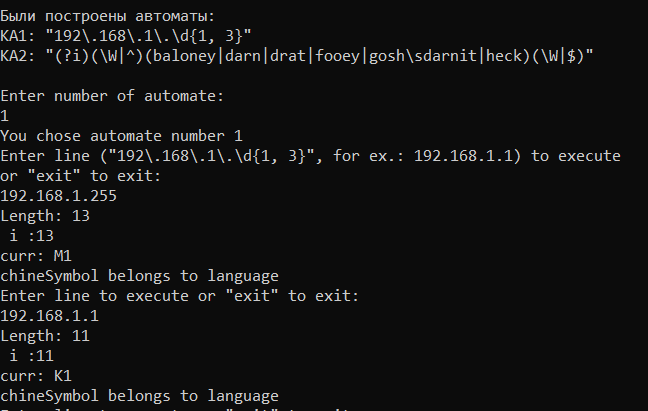
\includegraphics[]{3.png}
		\label{fig:mpr}
	\end{figure}
	\begin{figure}[h]
		\centering
		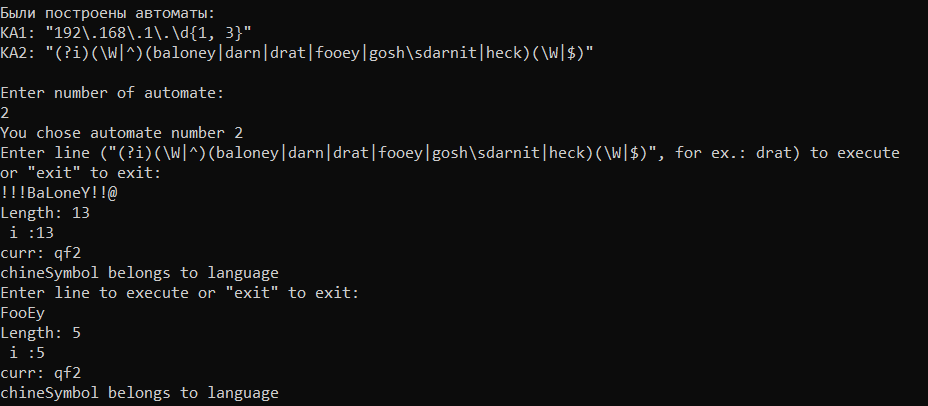
\includegraphics[]{4.png}
		\label{fig:mpr}
	\end{figure}
	
\end{document}